\documentclass{article}
\usepackage[spanish]{babel}
\usepackage{graphicx}

\title{Cómputo Concurrente 2024-2 \\ Práctica 2 \\  Ley de Amdahl y Paralelismo}

\author{Natalia Abigail Pérez Romero\\
Jonathan Bautista Parra \\ Valeria Reyes Tapia}

\date{\today}

\begin{document}

\maketitle
\section{Introduction}
En esta práctica se implementó un programa en Java que simula un ataque de fuerza bruta para obtener una contraseña. El programa utilizará hilos para realizar el ataque de manera concurrente de forma que cada hilo se encarga de buscar una parte de las combinaciones posibles de la contraseña. También se calculará la aceleración teórica y obtenida en función del número de hilos y porcentaje de código en paralelo.

\section{Graficas y tablas de valores}

Después de ejecutar la solución para 1, 2, 27 y 100 hilos, se obtuvieron los siguientes resultados:

\begin{table}[h]
    \centering
        \begin{tabular}{|c|c|}
            \hline
            \textbf{Número de hilos} & \textbf{Tiempo de ejecución (s)} \\
            \hline
            1 & 5.79159E+11\\
            \hline  
            2 &  7.2579E+11 \\
            \hline
            27 &  3.64659E+11\\
            \hline
            100 &  1.21143E+12\\
            \hline
        \end{tabular}
    \caption{Tabla de tiempos de ejecución en función del número de hilos.}
    \label{tab:tiempos-ejecucion}
\end{table}

\begin{figure}
    \centering
    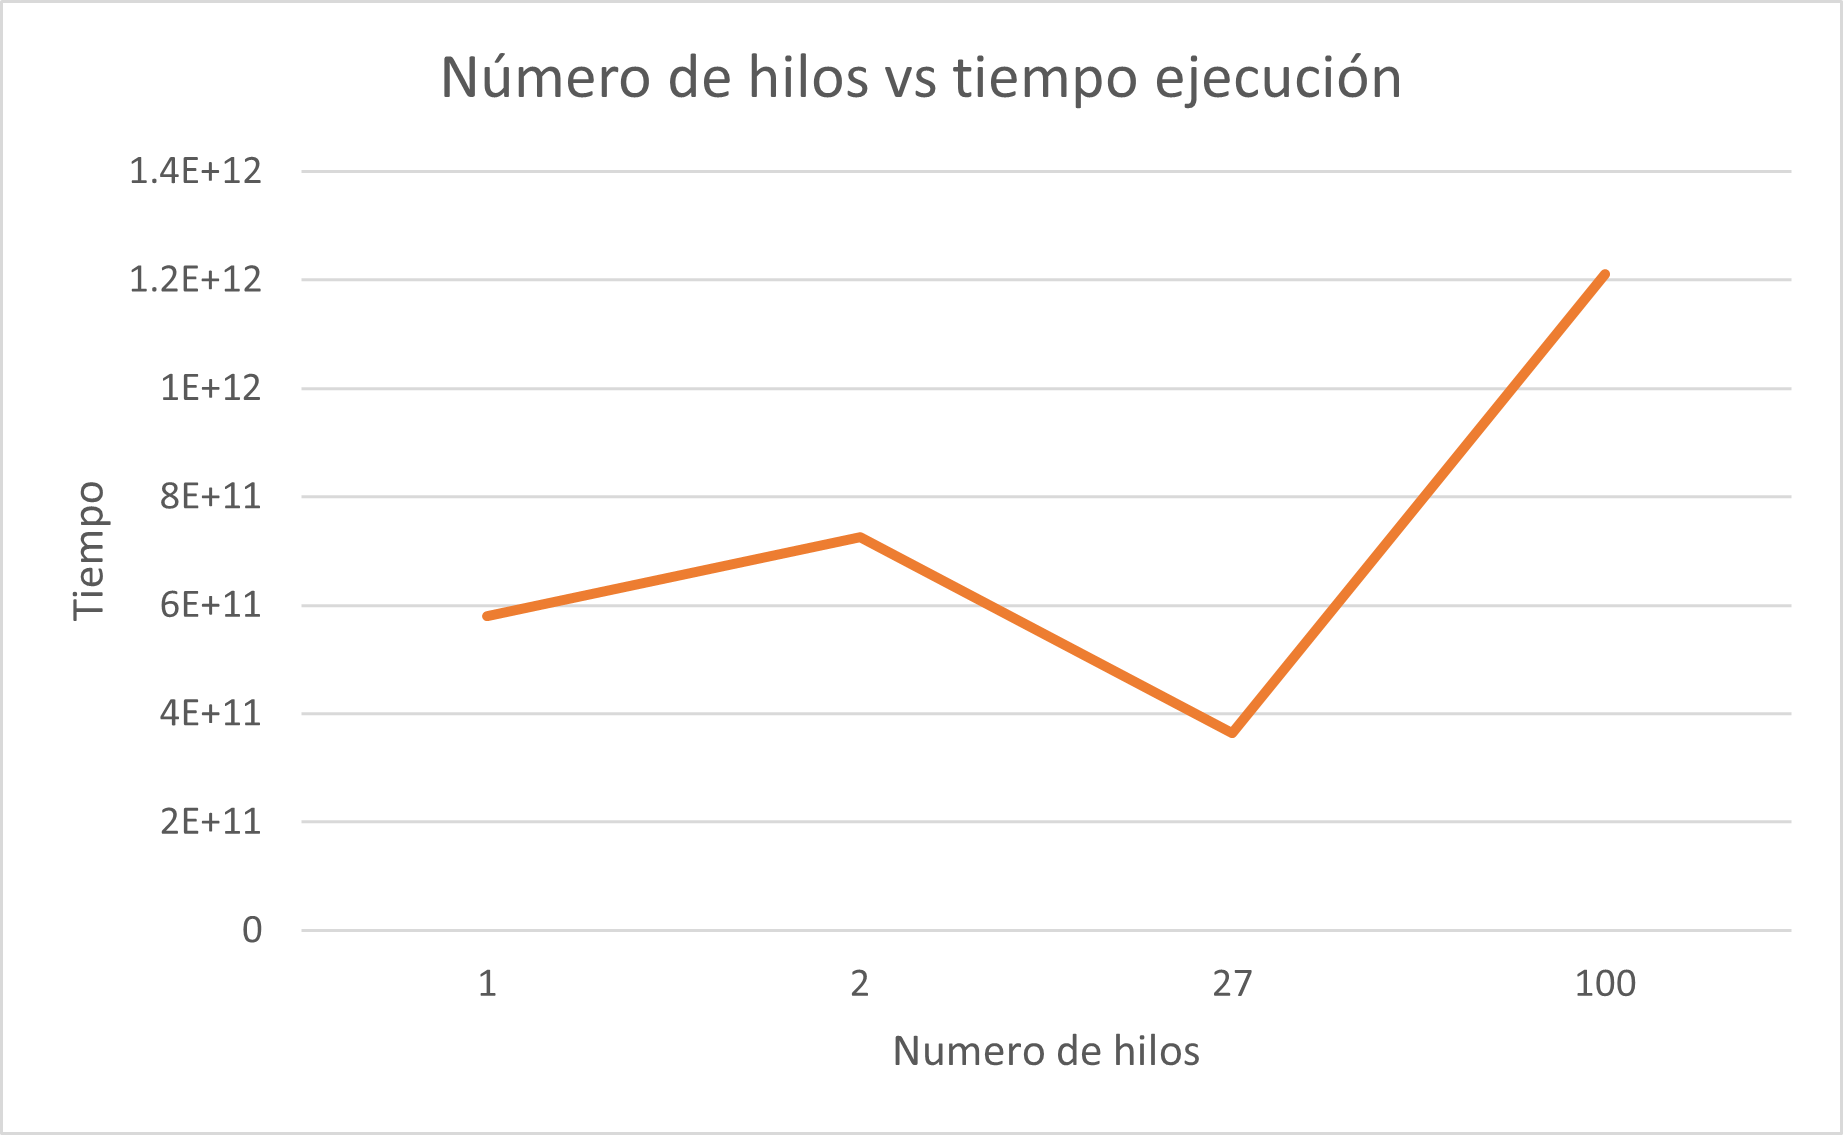
\includegraphics[width=\textwidth]{diagramaTiempoVSHilos.png}
    \caption{Gráfica de tiempos de ejecución en función del número de hilos.}
    \label{fig:tiempos-ejecucion}
\end{figure}


Nuestra contraseña tiene 6 caracteres, por lo que el número de combinaciones posibles es $26^6 = 308 915 776$. En la tabla \ref{tab:aceleracion-teorica-obtenida} se muestra la aceleración teórica y obtenida en función del número de hilos y porcentaje de código en paralelo.
En este caso, consideramos el porcentaje de código paralelizable como el $100\%$, dado que los hilos no requieren de comunicación entre ellos para realizar su trabajo.

\begin{table}[h]
\centering
\begin{tabular}{|c|c|c|c|}
\hline
\textbf{Número de} & \textbf{Aceleración} & \textbf{Aceleración} & \textbf{\% código} \\
\textbf{hilos} & \textbf{teórica} & \textbf{obtenida} & \textbf{en paralelo} \\
\hline
1 & 1 & 5.79159E+11 & 100 \% \\
2 & (5.79159E+11/2) = 2.8958E+11 & 7.2579E+11 & 100 \%  \\
27 & (5.79159E+11/26) = 2.14133E+10 & 3.64659E+11 & 100 \%  \\
100 & (5.79159E+11/100) = 2.14133E+10 & 1.21143E+12 & 100\% \\
\hline
\end{tabular}
\caption{Tabla de aceleración teórica y obtenida en función del número de hilos y porcentaje de código en paralelo.}
\label{tab:aceleracion-teorica-obtenida}
\end{table}
Si el tiempo de ejecución con un hilo es de 5.79159E+11, entonces la aceleración teorica con 2 hilos es de 2.89579E+11, con 27 hilos es de 2.14133E+10 y con 100 hilos es de 5.79159E+9.

\section{Cuestionario}
\begin{enumerate}
    \item ¿Cuál fue mi contraseña?
    
    La contraseña es: hlsbrr

    \item ¿Cuántas posibles contraseñas hay?

    Si la contraseña tiene entre 7 y 13 caracteres, por lo que el numero de combinaciones posibles es:
    \[ \Sigma_{i=7}^{i=13} 26^i = 2 147 583 647\]

    Nuestra contraseña es de 6 caracteres, por lo que el numero de combinaciones posibles es:
    \[ 26^6 = 308 915 776\]

    \item ¿La ley de Amdahl siempre se cumple?
    
    No. La ley de Amdahl no siempre se cumple en la práctica. La ley establece que la mejora de la velocidad de un componente de un sistema solo puede mejorar el rendimiento general del sistema hasta un límite determinado. El límite está determinado por la fracción del tiempo que se ejecuta el componente en cuestión.

    \item ¿En qué casos no se cumple?
    
    La introducción de paralelismo puede llevar la necesidad de sincronización entre hilos o procesos, la comunicación entre ellos y la gestión de recursos compartidos. Esto puede contrarrestar parcial o totalmente los beneficios del paralelismo. Problemas con dependencias de datos, donde la salida de una operación es necesaria como entrada para otra, pueden limitar la capacidad de paralelización. 
   
    \item ¿Por qué crees a que se debe esto?
    
    Los sistemas no son perfectamente paralelos: La mayoría de los sistemas tienen algunos componentes que son secuenciales.
    Los componentes no siempre se ejecutan al máximo rendimiento: Los componentes pueden estar inactivos o ejecutarse a una velocidad inferior a su máximo rendimiento.

    \item ¿Cuál sería la mejora máxima? Es decir, la aceleración teórica máxima
    
    La mejora máxima o aceleración teórica máxima según la Ley de Amdahl se puede calcular utilizando la fórmula proporcionada por la misma ley:
    \[S= \frac{1}{F_s-\frac{F_p}{P}}\]
    Donde:
    \begin{itemize}
        \item S es la mejora máxima
        \item $F_s$ es la fracción del código que se ejecuta de manera secuencial.
        \item $F_p$ es la fracción del código que se puede paralelizar.
        \item P es el número de procesadores
    \end{itemize}
    La mejora máxima se alcanza cuando P tiende a infinito, es decir, cuando se utiliza un número infinito de procesadores:
    \[S = \frac{1}{F_s}\]

    Este resultado muestra que la mejora máxima está inversamente proporcional a la fracción secuencial del código $(F_s)$ Cuanto menor sea $(F_s)$, mayor será la mejora máxima posible. 

    \item Escribe tus conclusiones, además de lo que aprendiste en esta práctica, contratiempos y descubrimientos que hubo durante su realización.
    
    En esta práctica aprendimos a utilizar hilos en Java y a calcular la aceleración teórica y obtenida en función del número de hilos y porcentaje de código en paralelo. Aprendimos que la ley de Amdahl no siempre se cumple en la práctica y que la mejora máxima o aceleración teórica máxima se alcanza cuando se utiliza un número infinito de procesadores. 

    Durante la realización de la práctica, tuvimos problemas con la implementación de los hilos porque nuestro poder de computo es límitado, así que nuestra contraseña tuvo que ser de 6 caracteres, lo que limitó el número de combinaciones posibles.
    
    \item ¿Cuál es su rol? 
    
    Nuestro rol es el de los hilos, los cuales se les encarga el trabajo de obtener por fuerza bruta la contraseña para obtener un mensaje secreto. 

    \item ¿Cuál es mi rol?
    
    Tu rol es el del despachador, el cual se encarga de repartir el trabajo entre los hilos.

    
\end{enumerate}

\subsection{Una captura de pantalla cuando agregaste tus palabras.}

\begin{figure}[h!]
    \centering
    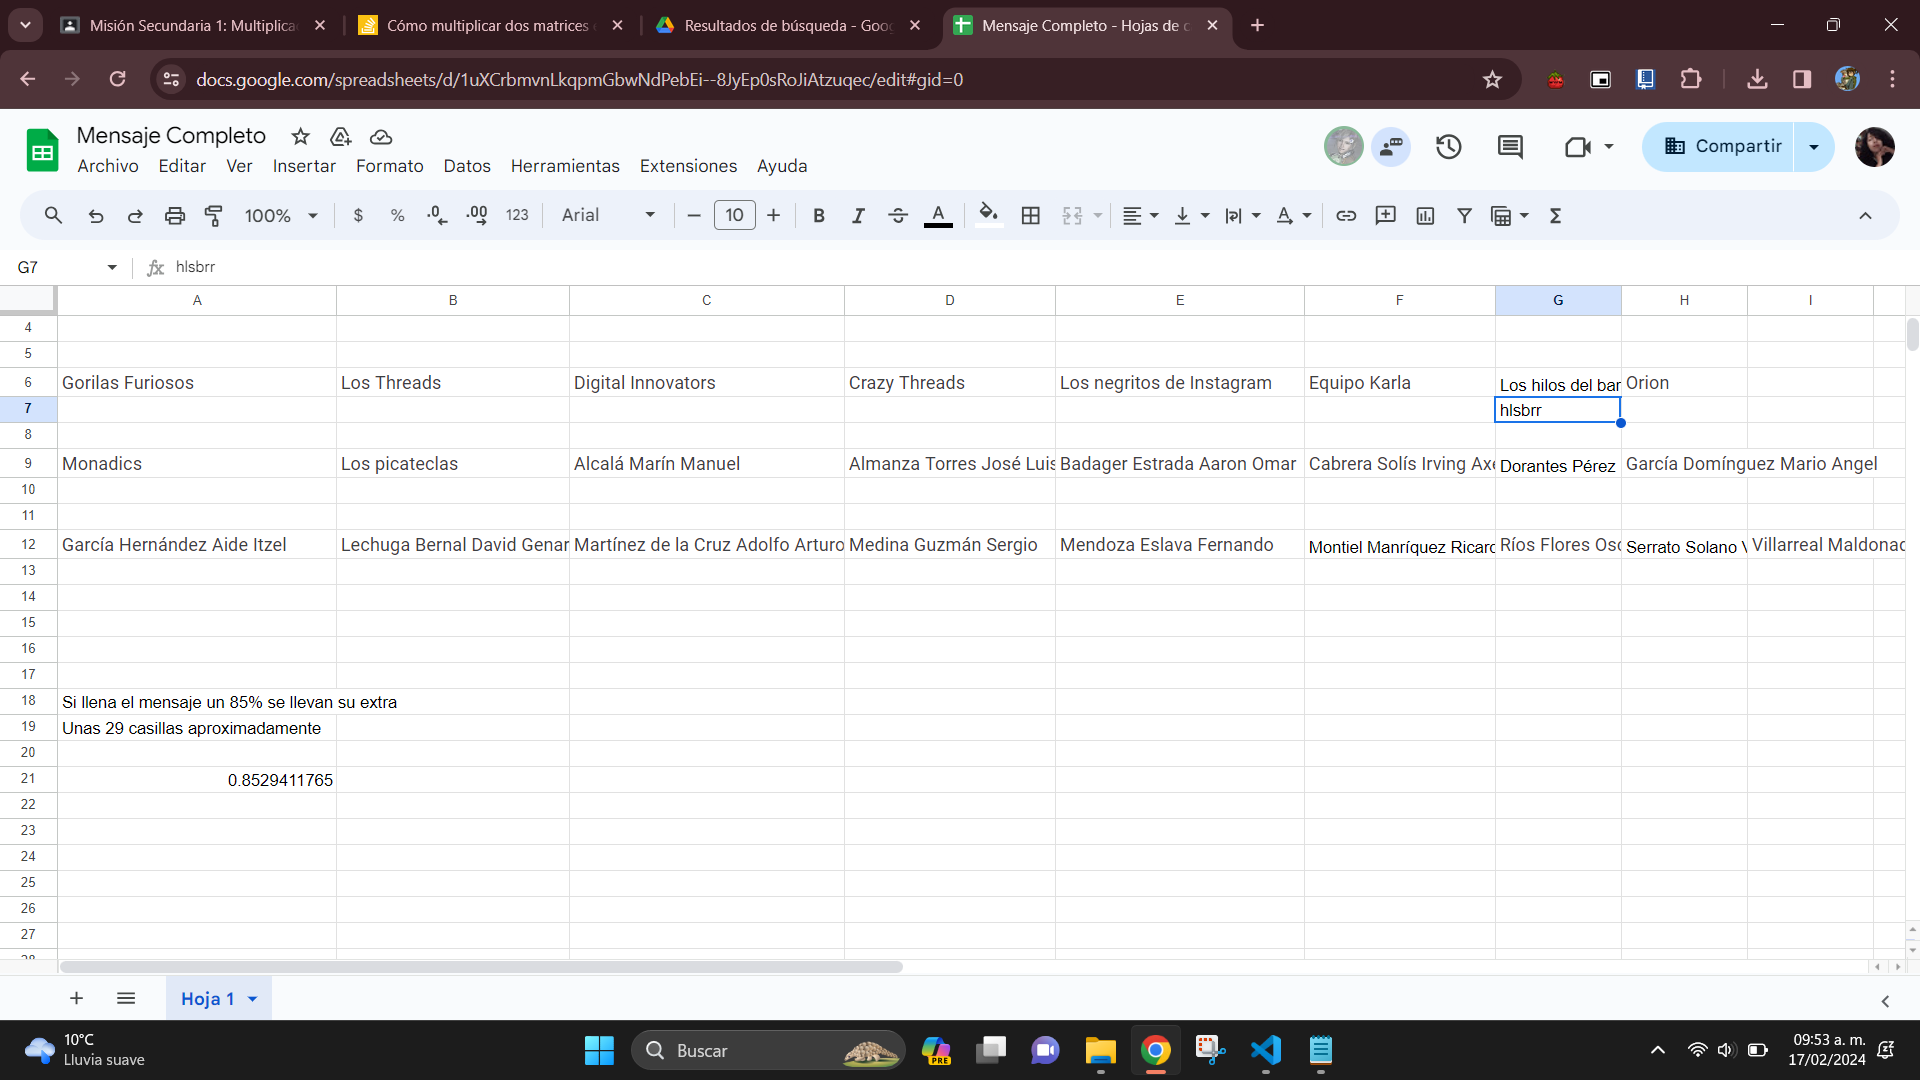
\includegraphics[width=\textwidth]{errorPalabra.png}
    \caption{Captura de pantalla de cuando se agregaron las palabras.}
    \label{fig:captura-pantalla}
\end{figure}

Corrección:
\begin{figure}[h!]
    \centering
    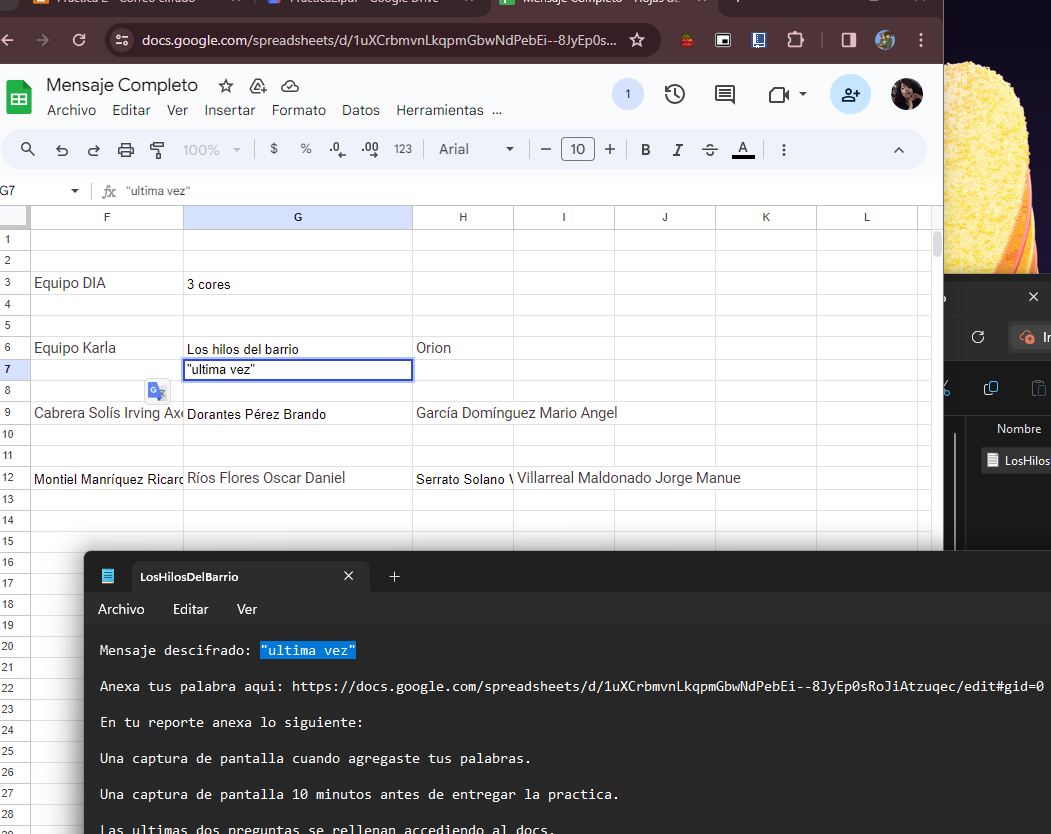
\includegraphics[width=\textwidth]{agreguePalabras.png}
    \caption{Captura de pantalla de cuando se agregaron las palabras.}
    \label{fig:captura-pantalla}
\end{figure}


\subsection{Una captura de pantalla 10 minutos antes de entregar la practica.}
\begin{figure}
    \centering
    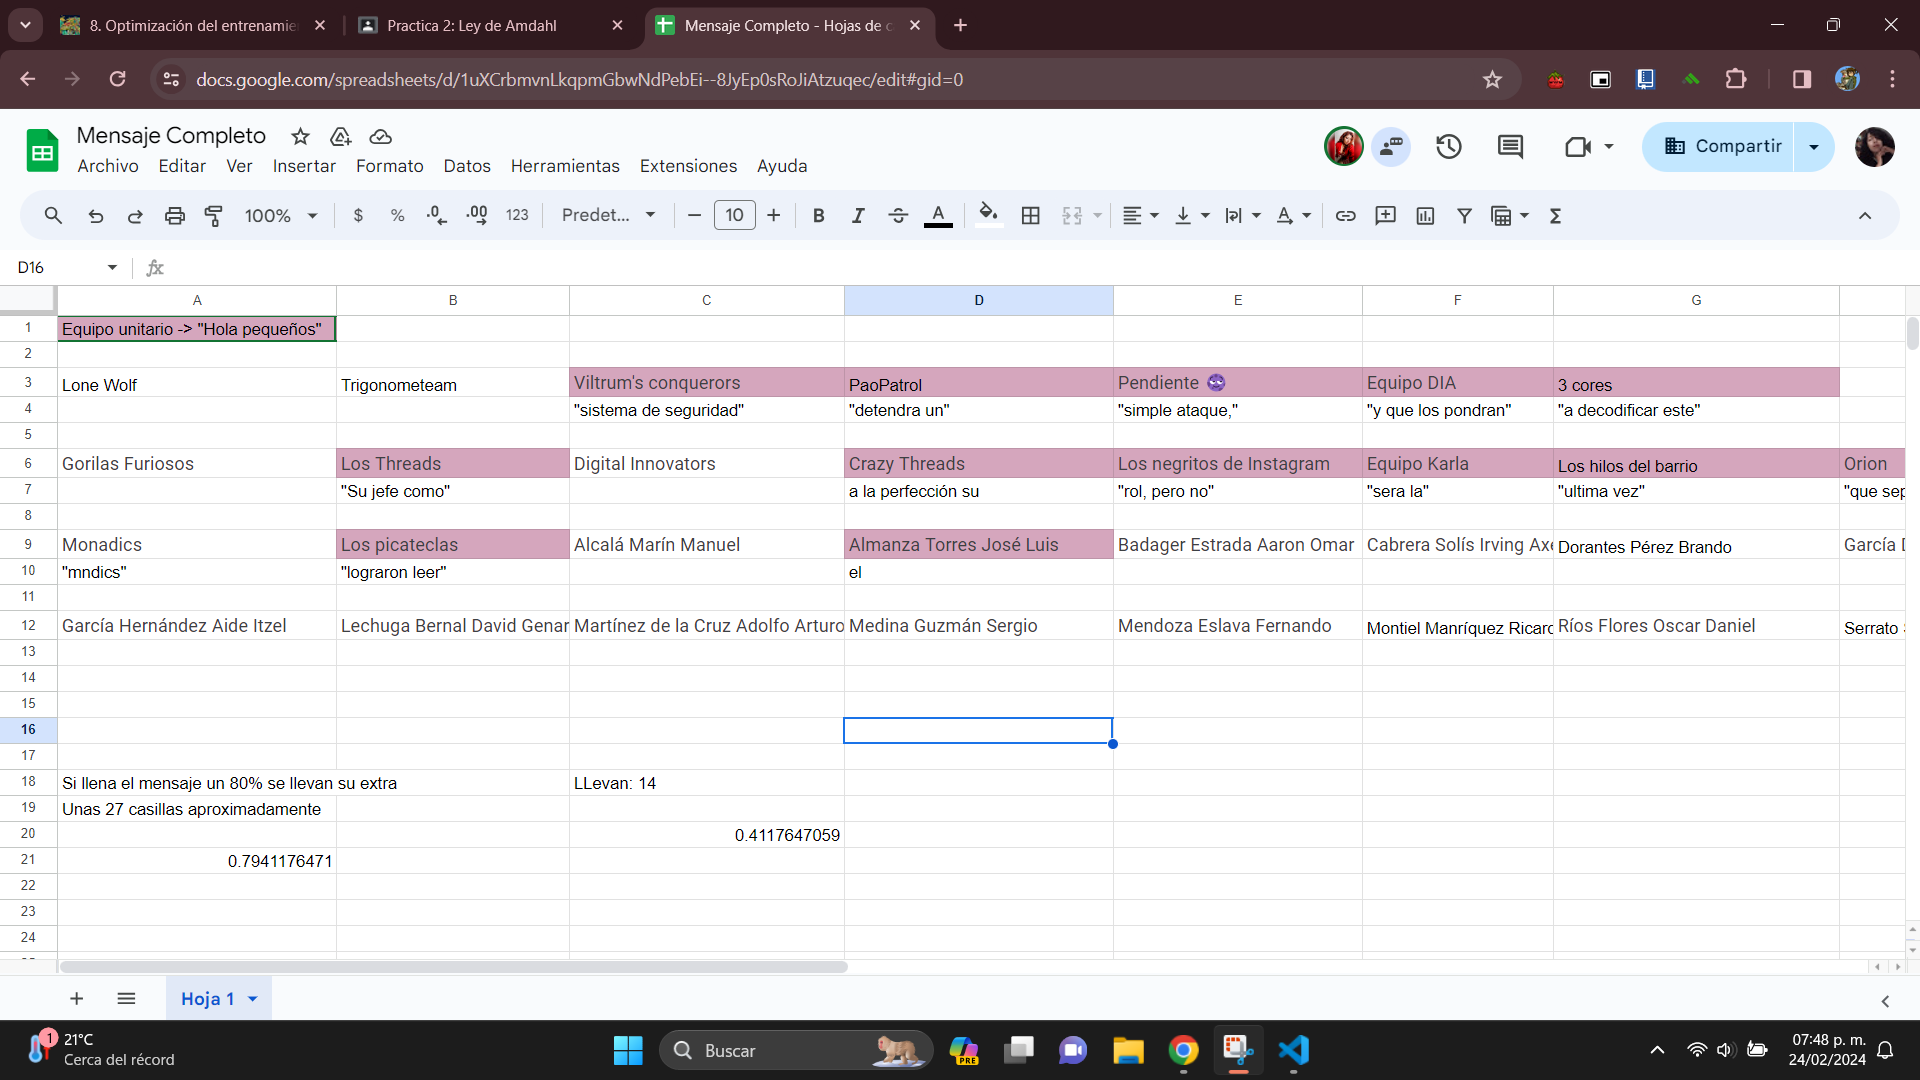
\includegraphics[width=\textwidth]{10minutos.png}
    \caption{Captura de pantalla 10 minutos antes de entregar la práctica.}
    \label{fig:captura-pantalla}
\end{figure}

\end{document}
